\section{Data Protection API (DPAPI)}

\href{https://docs.microsoft.com/en-us/previous-versions/ms995355(v=msdn.10)}{Data
ProtectionAPI (DPAPI)} is a simple cryptographic API available as a built-in component 

In theory, DPAPI enable symmetric encryption of any kind of data; in practice,
its primary {\bf use in the Windows operating system is to perform symmetric
encryption of asymmetric private keys, using a user or system secret as a
significant contribution of entropy}. A detailed analysis of DPAPI
inner-workings was published in 2011 by
\href{https://learn.microsoft.com/en-us/previous-versions/ms995355(v%3Dmsdn.10)}{Bursztein
et al}.

DPAPI allows developers to encrypt keys using a symmetric key derived from
the user's logon secrets, or in the case of system encryption, using the
system's domain authentication secrets.

DPAPI doesn't store any persistent data for itself; instead, it simply receives
plaintext and returns ciphertext (or conversely).

DPAPI security relies upon the Windows operating system's ability to protect
the master key and RSA private keys from compromise, which in most attack
scenarios is most highly reliant on the security of the end user's credentials.
A main encryption/decryption key is derived from user's password by PBKDF2
function. Particular data binary large objects can be encrypted in a way that
salt is added and/or an external user-prompted password (aka "Strong Key
Protection") is required. The use of a salt is a per-implementation option –
i.e. under the control of the application developer – and is not controllable
by the end user or system administrator.

Delegated access can be given to keys through the use of a COM+ object. This
enables IIS web servers to use DPAPI. 


PowerShell credentials are often used for scripting and automation tasks as a
way to store encrypted credentials conveniently. The credentials are protected
using DPAPI, which typically means they can only be decrypted by the same user
on the same computer they were created on.

\subsection{Process}
At a high level, for the user scenario, a user’s password is used to derive a
user-specific {\bf master key}. This master key needs to be decrypted using the
user’s password OR the domain backup key and is then used to decrypt any DPAPI
data blobs.

The encryption of user's personal data in DPAPI goes in three phases:
\begin{enumerate}
    \item 
        First, the application calls the CryptProtectData function, specifying the source data to be encrypted and the optional entropy parameter. If the latter is not specified, any other program in the context of current user may be able to decrypt the data by gaining physical access to the DPAPI blob.
    \item
        The CryptProtectData function belongs to the CryptoAPI family and is located in Crypt32.dll. From there, the request for further processing is forwarded via a secure RPC channel to the Local Security Authority (LSA) system process, and the context of current user is switched to the system. All the further manipulations are run in the context of the local system.
    \item 
        In the LSA, the data is actually encrypted and forwarded back to Crypt32.dll via the RPC channel; from there, the data safely travels to the original application.
\end{enumerate}

The encryption process: 
\begin{enumerate}
    \item 
        Derive the user's password by applying the PBKDB2 cryptographic standard to otain the \emph{Master Key encryption key}. 
    \item 
        use the \emph{Master key encryption key} to decrypt the \emph{Master Key}. 
    \item If the decryption fails, the user password is decrypted using the first hash of the credential history, CREDHIST, which in its turn also gets the Master Key encryption key and attempts to decrypt the Master Key again. If that attempt too ends up in failure, we decrypt the next credential history hash, and so on. The operation continues until either the Master Key is decrypted or the credential history runs out of its items.
\end{enumerate}

So, user's Master Key resides in a special container file, which can store additional copies - backups - of the Master Key. A Master Key backup is used when the primary copy, for one or the other reason, cannot be decrypted. For example, after a forced password reset. Master Key is a critical element in DPAPI cryptography; therefore, its length is 512 bits, and only proven algorithms are used when encrypting it.

Once the Master Key is successfully decoded, its source 512-bit data participates in obtaining the symmetric encryption key for the DPAPI blob.

For that purpose, the Master Key is "mixed" with random data (which would be then stored in the DPAPI blob) and entropy, if it is specified.

Stores another Master Key copy that was encrypted with the domain backup key. The domain backup key is an RSA key pair in which the private and public keys are stored in the Domain Controller (DC), and the public key is also distributed to every user’s profile, enabling each user to encrypt their own Master Key. This does not back up a copy of the Master Key to the DC, but provides the ability to recover it if the domain user’s password is forgotten. As there might be more than one domain backup key, this section includes a slot for the Guid of this key.

\subsection{Blob}

Blob can be stored on disk but also in regisrty and Active Directory

\begin{itemize}
    \item 
        contains: encrypted raw data, secret, by example Vault, Credential, CAPI/CNG
        Private Key, Chrome password, WiFi/WWAN key,\ldots
    \item 
        Is protected by: a {\bf master key} and optionally {\bf entropy data} AND/OR
        aditionnal {\bf password}
    \item 
        is linked to a {\bf master key}
\end{itemize}


\subsection{Master Keys}

When we navigate to the Master Key’s path, we may encounter more than one Master Key file. This is because Master Keys are set to expire after approximately 90 days from the day they were created.

The User's DPAPI master keys are stored under \verb+%APPDATA%\Microsoft\Protect\{SID}+ directory, where \verb+{SID}+ is the Security Identifier of that user. 

These files have the "System files" attribute, and so \verb+DIR /AS+ must be used

\begin{verbatim}
Get-ChildItem -Hidden C:\Users\USER\AppData\Roaming\Microsoft\Protect\
Get-ChildItem -Hidden C:\Users\USER\AppData\Local\Microsoft\Protect\

dir %appdata%\Microsoft\Protect\ /s 
dir %localappdata%\Microsoft\Protect\ /s 
\end{verbatim}

System's Master Keys are stored in \verb+%WINDIR%/System32/Microsoft/Protect+ and used for decrypting DPAPI blobs, protected under a local system account.

\begin{itemize}
    \item 
        contains: multiple versions of the encrypted raw key.
    \item 
        Is protected by: a key that depends on the situation
        \begin{itemize}
            \item non-domain context: SID AND (user password SHA1 hash OR previous
                password SHA1 hash (by knowledge or from CREDHIST))
            \item domain context: SID AND (user password NTLM hash OR previous password
                NTLM hash (by knowledge)) domain backup key (RPC or RSA private key)
            \item local computer: \verb+DPAPI_SYSTEM+ secret (COMPUTER or USER part)
        \end{itemize}
\end{itemize}

A user's Master Key is a binary file that contains encrypted data used for creating the primary encryption key in all DPAPI blobs.

\begin{figure}[!ht]
    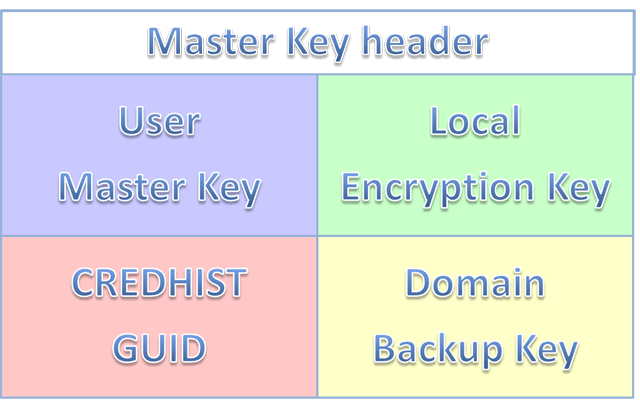
\includegraphics[width=\linewidth]{windows_knowledge/security/images/dpapi5.png}
  \caption{DPAPI Master key structur}
  \label{fig:dpapi-master-key-structure}
\end{figure}
As shown on Figure 4, a Master Key file consists of 5 units:
\begin{itemize}
    \item 
    Header and system information
    \item 
        User's Master Key: Stores the Master Key in a user-encrypted form, where the phrase used to encrypt it is the user’s password or \verb+DPAPI_SYSTEM+ registry key (depending on the authority).
    \item 
    Local backup encryption key: This legacy section, used in Windows 2000, stores a local encryption key to decrypt a local backup of the Master Key; in Windows 2000. This section is not in use from Windows 2K3/XP versions, but still contains data.
    \item 
    Unique CREDHIST file identifier: Stores a Guid that points to a link stored in the user’s CREDHIST file. The CREDHIST (Credential History) file maintains a chain of a local user password history, in an encrypted form. As local users may change their passwords, DPAPI requires the ability to read the password that was used to encrypt a Master Key created in the past.
    \item 
    Domain Master Key backup: Stores another Master Key copy that was encrypted with the domain backup key. The domain backup key is an RSA key pair in which the private and public keys are stored in the Domain Controller (DC), and the public key is also distributed to every user’s profile, enabling each user to encrypt their own Master Key. This does not back up a copy of the Master Key to the DC, but provides the ability to recover it if the domain user’s password is forgotten. As there might be more than one domain backup key, this section includes a slot for the Guid of this key.
\end{itemize}

\begin{figure}[!ht]
    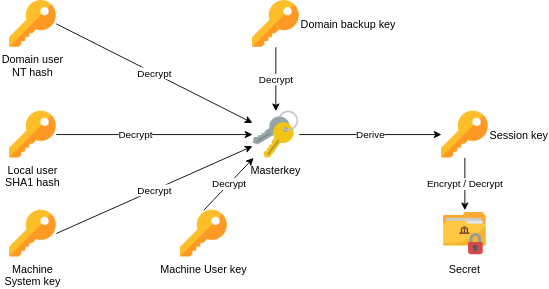
\includegraphics[width=\linewidth]{windows_knowledge/security/images/dpapi4.png}
    \caption{DPAPI Master keys}
  \label{fig:dpapi-master-keys}
\end{figure}

The masterkey decryption will have different prerequisites depending on the context, as shown in the previous diagram:

\begin{itemize}
    \item 
        Domain user: its password or NT hash, or the domain backup key.
    \item
        Local user: its password or SHA1 hash.
    \item
        Local DPAPI: both systemand security hives to compute the key.
\end{itemize}

{\bf Moreover, masterkeys can also be used to perform offline brute force of a user's password using John The Ripper}

\subsection{DPAPI Credential History}

The proper functioning of DPAPI assumes keeping all of user's previous passwords. All the previous passwords are stored as hashes in a special container file named \verb+CREDHIST+, located in the \verb+%APPDATA%/Microsoft/Protect folder+.

If we look at the credential history file as a chain, each slot with a password hash would appear as a link of the chain.

Slots with user's hashes are stored in series, one after another. Each password hash is encrypted with the preceding hash, and the first hash is encrypted with user's current password. Therefore, to decrypt the entire chain, one needs to know user's current password.

If an error occurs when decrypting the Master Key using current password, DPAPI uses the logon password to decrypt the first hash in CREDHIST and attempts to decrypt the Master Key with the first CREDHIST hash. If the Master Key still resists, the first hash in the CREDHIST history decrypts the second hash, and the operation repeats. 

Different operating systems use different default parameters and algorithms for encrypting credential history.


\subsection{Password change}

Password change in Windows is conventionally divided into several critical phases. First, the system checks the validity of the old password, then checks the new password for compliance with security policies and physically changes the password in the SAM or NTDS.DIT databases. In the second phase, if all goes well, it updates the internal password cache. Then there runs the DPAPI password change routine. And, finally, it updates the biometric logon credential for the user.

The DPAPI system is smart enough to handle various scenarios:




\subsection{Backup key dumps}

\href{https://www.sygnia.co/blog/the-downfall-of-dpapis-top-secret-weapon/}{The Downfall Of Dpapi Top Secret Weapon}
The purpose of the domain backup process is to enable domain users to recover their Master Keys in case they forget their password. Unlike local users, who maintain a CREDHIST file, a domain user’s password might be set from the Active Directory in a password reset scenario. In that case, when the domain user logs back in using the new password, DPAPI will not be able to decrypt any Master Key, and will thus start the Master Key recovery process, using the MS-BKRP protocol.
During the recovery process, DPAPI takes the data from ‘Section 4: Domain Backup’ (\verb+MASTERKEY_DOMAINKEY+) of the Master Key, and sends it to the DC over a secured RPC call, utilizing the MS-BKRP protocol. The DC decrypts the data sent by the user, and validates that the user owns this key. Finally, the DC returns the unencrypted Master Key value so that DPAPI can re-encrypt ‘Section 1: User encrypted Master Key’ of all Master Keys files with the new user’s password:


To put this recap in a nutshell: top secret data associated with domain users is encrypted with each user’s ‘preferred’ Master Key. Each Master Key is protected in two different ways: with the user’s password, and with the domain backup key. This means that secrets protection is only as robust as the user’s password or the backup key being used. Users’ passwords can be changed … but what about the domain backup key we all trust?

The backup key is stored in the Active Directory as an LSA secret object, and is replicated across all Domain Controllers in the same domain. Members of the Domain Administrators group have the required privileges to read this key, and tools like Mimikatz and SharpDPAPI can aid in automating the dump process and conversion of the key to a PVK format. The PVK can be later used to decrypt a Master Key of any user in the domain.

The backupkey command will retrieve the domain DPAPI backup key from a domain controller using the LsaRetrievePrivateData API approach from Mimikatz. This private key can then be used to decrypt master key blobs for any user on the domain. And even better, the key never changes ;)

Domain admin (or equivalent) rights are needed to retrieve the key from a remote domain controller.

\subsubsection{Method 1 – LSA remote protocol [ms-lsad]}

From the perspective of an adversary, Mimikatz is a great tool to dump the backup key secrets into an operatable format. First, it gets the preferred GUID identifier of the backup key; then, it dumps the secret contents and re-assembles the key pair into PVK and PFX formats. It also takes the certificate part of the backup key and exports it to a DER-formatted file. For the legacy key, Mimikatz just exports the key contents.

The operation shown above is done through a protocol named MS-LSAD. This protocol allows interacting with AD secret objects, where section 3.1.4.6.6 (LsarRetrievePrivateData) specifies the operation used to extract the data of a secret (such as the backup key). The SharpDPAPI tool dumps the backup key contents in the same way.

\subsubsection{Method 2 - ntds.dit}

Another way to get the backup key content is by dumping the NTDS.dit database. As the backup key is an Active Directory object, it will also be included within its database.

Once the operation is completed, we can go offline and use the DSInternals framework with the ‘SYSTEM’ hive and NTDS.dit database, to extract the backup key and re-assemble it to PFX and PVK formats.



\subsection{links}
\begin{itemize}
    \item 
        \href{https://www.passcape.com/index.php?section=docsys&cmd=details&id=28#13}{DPAPI Secrets}
    \item
        \href{https://www.synacktiv.com/publications/windows-secrets-extraction-a-summary}{Windows secrets extraction: a summary}
        
\end{itemize}


